\documentclass{beamer}
\mode<presentation>
\usepackage{amsmath}
\usepackage{amssymb}
\usepackage{bm}
%\usepackage{advdate}
\usepackage{adjustbox}
\usepackage{subcaption}
%\usepackage{enumitem}
\usepackage{enumerate}
\usepackage{multicol}
\usepackage{mathtools}
\usepackage{listings}
\usepackage{url}
\def\UrlBreaks{\do\/\do-}
\usetheme{Boadilla}
\usecolortheme{lily}
\setbeamertemplate{footline}
{
  \leavevmode%
  \hbox{%
  \begin{beamercolorbox}[wd=\paperwidth,ht=2.25ex,dp=1ex,right]{author in head/foot}%
    \insertframenumber{} / \inserttotalframenumber\hspace*{2ex} 
  \end{beamercolorbox}}%
  \vskip0pt%
}
\setbeamertemplate{navigation symbols}{}

\providecommand{\nCr}[2]{\,^{#1}C_{#2}} % nCr
\providecommand{\nPr}[2]{\,^{#1}P_{#2}} % nPr
\providecommand{\mbf}{\mathbf}
\providecommand{\pr}[1]{\ensuremath{\Pr\left(#1\right)}}
\providecommand{\qfunc}[1]{\ensuremath{Q\left(#1\right)}}
\providecommand{\sbrak}[1]{\ensuremath{{}\left[#1\right]}}
\providecommand{\lsbrak}[1]{\ensuremath{{}\left[#1\right.}}
\providecommand{\rsbrak}[1]{\ensuremath{{}\left.#1\right]}}
\providecommand{\brak}[1]{\ensuremath{\left(#1\right)}}
\providecommand{\lbrak}[1]{\ensuremath{\left(#1\right.}}
\providecommand{\rbrak}[1]{\ensuremath{\left.#1\right)}}
\providecommand{\cbrak}[1]{\ensuremath{\left\{#1\right\}}}
\providecommand{\lcbrak}[1]{\ensuremath{\left\{#1\right.}}
\providecommand{\rcbrak}[1]{\ensuremath{\left.#1\right\}}}
\providecommand{\rank}{\text{rank}}
\theoremstyle{remark}
\newtheorem{rem}{Remark}
\newcommand{\sgn}{\mathop{\mathrm{sgn}}}
\providecommand{\abs}[1]{\left\vert#1\right\vert}
\providecommand{\res}[1]{\Res\displaylimits_{#1}} 
\providecommand{\norm}[1]{\lVert#1\rVert}
\providecommand{\mtx}[1]{\mathbf{#1}}
\providecommand{\mean}[1]{E\left[ #1 \right]}
\providecommand{\fourier}{\overset{\mathcal{F}}{ \rightleftharpoons}}
%\providecommand{\hilbert}{\overset{\mathcal{H}}{ \rightleftharpoons}}
\providecommand{\system}{\overset{\mathcal{H}}{ \longleftrightarrow}}
	%\newcommand{\solution}[2]{\vec{Solution:}{#1}}
%\newcommand{\solution}{\noindent \vec{Solution: }}
\providecommand{\dec}[2]{\ensuremath{\overset{#1}{\underset{#2}{\gtrless}}}}
\newcommand{\myvec}[1]{\ensuremath{\begin{pmatrix}#1\end{pmatrix}}}
\newenvironment{amatrix}[1]{%
  \left(\begin{array}{@{}*{#1}{c}|c@{}}
}{%
  \end{array}\right)
}
\let\vec\mathbf

\lstset{
%language=C,
frame=single, 
breaklines=true,
columns=fullflexible
}

%\numberwithin{equation}{section}

\title{Matgeo-q 2.3.2}
\author{Harichandana Varanasi-ai25btech11039}

\date{\today} 
\begin{document}

\begin{frame}
\titlepage
\end{frame}

\section*{Outline}

\begin{frame}
\frametitle{Question}
\textbf{Q.}\; Find the angle between unit vectors $\vec a$ and $\vec b$ such that $\sqrt{3}\,\vec a-\vec b$ is also a unit vector.

\end{frame}
%
\begin{frame}
\frametitle{Solution}

\textbf{Solution.}
\textbf{Given:} $\|\vec{a}\|=\|\vec{b}\|=1$ and $\bigl\|\sqrt{3}\,\vec{a}-\vec{b}\bigr\|=1$.

\medskip
Use the length definition $\|x\|^2=x^\top x$ and the scalar–product relation $\vec{a}^\top\vec{b}=\|\vec{a}\|\,\|\vec{b}\|\cos\theta$.

\medskip
\[
\begin{aligned}
1
&=\bigl\|\sqrt{3}\,\vec{a}-\vec{b}\bigr\|^{2}\\
&=(\sqrt{3}\,\vec{a}-\vec{b})^\top(\sqrt{3}\,\vec{a}-\vec{b})\\
&=3\,\vec{a}^\top\vec{a}+\vec{b}^\top\vec{b}-2\sqrt{3}\,\vec{a}^\top\vec{b}\\
&=3\cdot 1+1\cdot 1-2\sqrt{3}\,\cos\theta\\
&=4-2\sqrt{3}\,\cos\theta.
\end{aligned}
\]
Hence $\,2\sqrt{3}\,\cos\theta=3\,$, so $\displaystyle \cos\theta=\frac{\sqrt{3}}{2}\,$ and therefore $\boxed{\theta=30^\circ}$.



\end{frame}
\begin{frame}{Plot}
    \begin{figure}[h!]
\centering
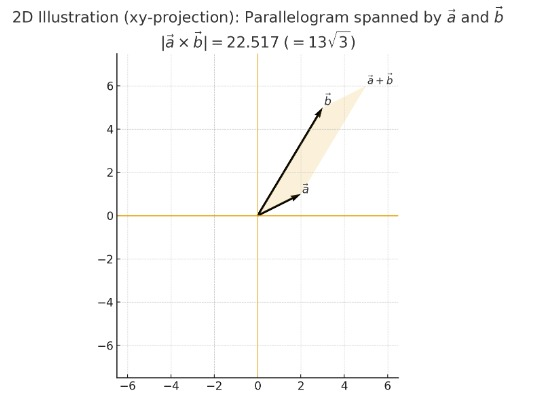
\includegraphics[width=0.7\linewidth]{figs/matgeo2.3.2.jpeg}
\caption{xy-projection of $\vec a$ and $\vec b$; $|\vec a\times\vec b|=13\sqrt{3}$.}

\end{figure}
\end{frame}
\end{document}
